%% Hvis gravitationelle bølger

% \section{Gravitationelle bølger}
% Den helt store svaghed ved den specielle relativitetsteori er, at den kun behandler inertialsystemer.
% I den Newtonske mekanik håndteres ikke-inertielle referencesystemer ved at introducere inertielle kræfter\footnote{Også kaldet fiktive kræfter.}.
% Den simpleste af disse er elevatorkræften der opleves ved konstant acceleration.
% \begin{equation}
%     F_\text{elevator}=ma
% \end{equation}
% hvor $a$ er systemets acceleration.
% Bemærk at elevatorkraften på et legeme afhænger af legemets masse.
% Dette gælder for alle inertielle kræfter, men også for tyngdekraften.
% Denne erkendelse ledte Einstein til ækvivalensprincippet:
% \begin{quote}
%     Der er 
% \end{quote}


%% Hvis lyskeglen

\subsubsection{Lyskeglen} \label{sec:Lyskeglen}
Vi så i afsnit \ref{rel:samtidighed}, at forskellige observatører ikke vil være enige om, hvorvidt to begivenheder sker samtidigt.
Vi har dog lige set, at begivenhederne vil have samme rumtidsinterval for alle observatører.
Lad os starte med at se på to begivenheder, der er samtidige i et inertialsystem, $S$.
Dette er ensbetydende med at 
$$
\Delta t^2=0 \: .
$$
I dette tilfælde er rumtidsintervallet
$$
\Delta s^2 = \Delta x^2\geq 0 \: .
$$
Når rumtidsintervallet er større end nul, siges de to begivenheder at være \emph{rumadskilte}.
I den modsatte situation, hvor der er et inertialsystem, hvor de to begivenheder sker samme sted, har vi
$$
\Delta x^2=0 \: ,
$$
hvilket medfører, at
$$
\Delta s^2=-c^2\Delta t^2\leq 0 \: .
$$
Når rumtidsintervallet er mindre end nul, siges begivenhederne at være \emph{tidsadskilte}.
Det efterlader en situation, når rumtidsintervallet er lig nul.
Det svarer til, at
$$
\Delta x^2=c^2\Delta t^2 \: ,
$$
hvilket kan skrives som
$$
\frac{\Delta x}{\Delta t}=\pm c \: .
$$
Rumtidsintervallet er således nul for begivenheder, som vi kan forbinde med en lysstråle.
Af denne grund kaldes dette, at de to begivenheder er \emph{lysadskilte}.

\begin{figure}
    \centering
    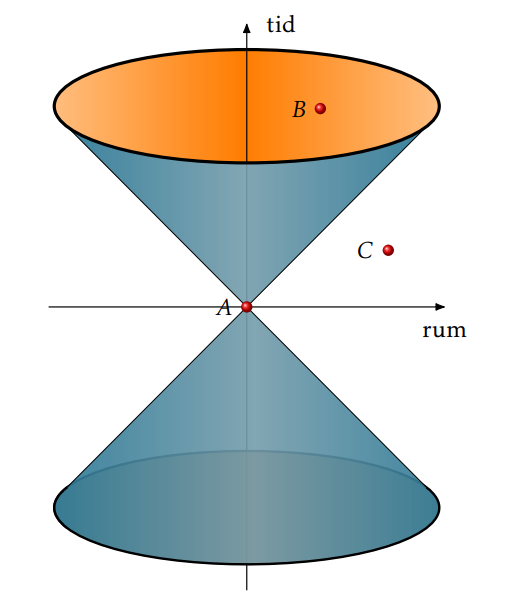
\includegraphics[width = 0.6\textwidth]{SR/billeder/lyskeglen.png}
    \caption{Lyskeglen med 2 rum dimensioner og en tidsdimension. Begivenhed \textrm{B} ligger i fremtiden for begivenhed \textrm{A}, mens begivenhed \textrm{C} ligger andetsteds. Kilde: figur~11.1 i \cite{uggerhojSpecielRelativitetsteori2016}.}
    \label{fig:lyskeglen}
\end{figure}

Hvis man laver et diagram med en $x$-akse og en $ct$-akse, vil lysstråler være linjer med en $45^\circ$'s vinkel til begge akser, der skærer i $(0,0)$, hvilket er beskrevet ved ligningen
%
\begin{subequations} \label{eq:lyskegle}
    %
    \begin{align} \label{eq:lyskegle_1d}
        0 = \Delta x^2 - c^2\Delta t^2
    \end{align}
    %
    Tilføjes en ekstra rummelig dimension er lyskeglen beskrevet af ligningen
    %
    \begin{align} \label{eq:lyskegle_2d}
        0 = \Delta x^2 + \Delta y^2 - c^2\Delta t^2
    \end{align}
    %
    og svarer ligningen nu til keglen i figur \ref{fig:lyskeglen}, hvorfor et sådant diagram kaldes en lyskegle. 
    Tilføjer man den resterende rumakse fås ligningen
    %
    \begin{align} \label{eq:lyskegle_3d}
        0 = \Delta x^2 + \Delta y^2 + \Delta z^2 - c^2\Delta t^2
    \end{align}
    %
    Der er nu fire parametre, hvorfor der skal bruges et firedimensionelt rum til at tegne ligningen, der nu tager form af det man kalder en hyperkegle\footnote{En hyperkegle er en figur, der konstrueres på samme måde som en kegle i 4 dimensioner. På samme måde er en kugle en hypercirkel, da det er den tredimensionelle udgave af cirkelen.}, hvilket ikke hjælper synderligt med visualiseringen. Rent matematisk er ligning \eqref{eq:lyskegle_3d} ikke mere særlig end de to andre. Den har bare ikke den praktiske egenskab at den kan tegnes på samme måde som ligning \eqref{eq:lyskegle_1d} og \eqref{eq:lyskegle_2d}, men det gør ikke matematikken forkert.
\end{subequations}
% Vi kan dog få et godt indblik, hvis vi har to rummelige dimensioner og en tidslig dimension.
% Så danner lysstrålerne en kegle omkring tidsaksen, se figur \ref{fig:lyskeglen}.
Denne {\em lyskegle} indeler rumtiden i tre forskellige områder.
\begin{itemize}
    \item \emph{Fremtiden} er alt det, der ligger indenfor keglen, men længere ud af tidsaksen end origo. Alle begivenheder, der ligger her, sker senere for en observatør i origo. På figur \ref{fig:lyskeglen} er ''B'' en fremtidig begivenhed for begivenhed ''A''.
    \item \emph{Fortiden} er alt det, der ligger indenfor keglen, men længere tilbage af tidsaksen end origo. Alle begivenhederne her er sket tidligere for en observatør i origo.
    \item Udenfor keglen er \emph{andetsteds}, dvs. begivenheder, som en observatør i origo og en ved andetstedsbegivenheden ikke kan blive enige om, er sket før, samtidig med eller vil ske efter hinanden. En andetstedsbegivenhed og begivenheden i origo kan altså ikke påvirke hinanden, da det ville kræve en påvirkning med overlyshastighed. På figur \ref{fig:lyskeglen} er begivenhed ''C'' andetsteds i forhold til begivenhed ''A''.
\end{itemize}
Vi tegner altså altid lyskeglen ud fra den begivenhed, på figur \ref{fig:lyskeglen} er det ''A'', som vi ønsker at forholde andre begivenheder til.

Ovenfor har vi kigget på fremtidige og fortidige begivenheder, samt begivenheder udenfor lyskeglen selv. De første to typer af begivenheder kaldes tidsadskilte begivenheder, mens den sidstnævnte kaldes en rumadskilt begivenhed. Om disse typer begivenheder kan det vises, ved brug af Lorentztransformationerne, at
\begin{quote}
    \emph{tidsadskilte} begivenheder kan \emph{rumligt} ombyttes og kan ske på samme sted, afhængigt af observatørens bevægelse, men rækkefølgen på begivenhederne kan ikke ændres,
\end{quote}
og
\begin{quote}
    \emph{rumadskilte} begivenheder kan \emph{tidsligt} ombyttes og kan ske til samme tid, afhængigt af observatørens bevægelse.
\end{quote}
Ligesom tidsadskilte begivenheders tidlige rækkefølge er ens for alle observatører, så kan man ikke bytte om på positionerne af rumligt adskilte begivenheder, da det ville ændre fortegnet på $\Delta x^2$ og dermed gøre begivenhederne tidsadskilte, hvilket ikke kan lade sig gøre. \\

Ideen med lyskeglen er at den gør det muligt at tegne sig ud af mange ting. Man kan hurtigt danne sig et overblik over hvilke begiverheder, der kan foregå på samme sted, og hvilke der kan foregå på samme tid og man kan åbne viden om rumtidsintervallets størrelse. Yderligere kan man også sige noget om hvilke begivenheder, der kan have noget med hinanden at gøre -- hvilket også kaldes korrelerede begivenheder. Tænkes tilbage til Einsteinsynkroniseringen af to ure, afsnit \ref{sec:sync}, så var der tale om fire begivenheder:
\begin{enumerate}
    \item ur A udsender et lysglimt
    \item ur B modtager lysglimtet fra A
    \item B udsender et lysglimt
    \item A modtager lysglimtet fra B
\end{enumerate}
I ur B's inertialsystem udsender B sit lysglimt samtidig med at det modtager lysglimtet fra A og da begge dele sker på samme sted, så må begivenhed 2. og 3. være lysadskilte med rumtidsinterval $\Delta s^2 = 0$, hvorfor disse begivenheder er samtidige for alle observatører. Begivenhed 2. kan først finde sted, når begivenhed 1. har fundet sted. Deres rækkefølge kan ikke ombyttes, hvorfor de må være tidsligt adskilte og tilsvarende med begivenhederne 3. og 4.